\documentclass[10pt,a4paper]{article}

\usepackage{fontspec}
\usepackage[french]{babel}
\usepackage[margin=1.6cm,top=1.3cm,bottom=1.5cm]{geometry}
\usepackage{amsmath}
\usepackage{array}
\usepackage{booktabs}
\usepackage{tabularx}
\usepackage{graphicx}
\usepackage{xcolor}
\usepackage{enumitem}
\usepackage{titlesec}
\usepackage{microtype}
\usepackage{tikz}
\usetikzlibrary{arrows.meta,positioning}
\usepackage[hidelinks]{hyperref}

\definecolor{accent}{HTML}{1F4E79}
\titleformat{\section}{\normalsize\bfseries\color{accent}}{\thesection.}{0.4em}{}
\titlespacing*{\section}{0pt}{5pt}{2pt}
\setlist{nosep,leftmargin=1.1em}
\setlength{\parindent}{0pt}
\setlength{\parskip}{2.5pt}
\setlength{\emergencystretch}{2em}
\pagestyle{empty}

\newcommand{\code}[1]{\texttt{#1}}
\newcolumntype{Y}{>{\raggedright\arraybackslash}X}

\begin{document}

\begin{center}
  {\Large\bfseries\color{accent} Compression d'image par DCT et stockage CSR en C++}\\[3pt]
  Romain \textsc{Ben}, Karim \textsc{Zrig} \quad|\quad MAM4 Polytech Nice Sophia, projet C++ \quad|\quad septembre 2026\\[1pt]
  {\small Code source : \url{https://github.com/BnRomain/jpeg-compression}, dossier \code{cpp/}}
\end{center}

\section{Objectif}
En MAM3, nous avions programmé en Python une compression d'image inspirée de JPEG,
avec un module de calcul (\code{jpeg\_compression.py}) et une application Streamlit :
DCT sur des blocs $8\times8$, quantification, suppression des hautes fréquences et
stockage creux au format CSR avec \code{scipy}. Ce projet réécrit l'ensemble en
C++20, sans bibliothèque de calcul, en s'appuyant sur les notions du cours. Le
programme en ligne de commande \code{jpeg\_csr} lit une image PNG ou JPEG, la
compresse, écrit les trois matrices CSR dans un fichier binaire \code{.csr},
reconstruit l'image et affiche les indicateurs de l'application Python (taux de
conservation, erreur, tailles mémoire). Les analyses du rapport MAM3 sont disponibles
par options : facteur de qualité $\alpha$, matrices $Q$ alternatives, troncature
carrée (version Python) ou triangulaire (sujet), bruit poivre et sel.

\section{Algorithme}
Pour chaque canal R, G, B et chaque bloc $M$ d'intensités centrées dans $[-128,127]$ :
\[
  D = P\,M\,P^{T}, \qquad P_{k,i} = \frac{C_k}{2}\cos\frac{(2i+1)k\pi}{16}, \qquad
  \hat D_{k,l} = \operatorname{trunc}\!\Big(\frac{D_{k,l}}{\alpha\,Q_{k,l}}\Big),
\]
avec $C_0 = 1/\sqrt{2}$ et $C_k = 1$ sinon. $\hat D_{k,l}$ est ensuite annulé si
$|\hat D_{k,l}| < S$ (seuil) ou si le masque le rejette : le masque carré garde
$k,l < F$, le masque triangulaire $k+l < F$. Les coefficients d'un canal forment une
matrice presque vide, stockée en CSR (valeurs \code{int16}, indices de colonnes et
pointeurs de lignes \code{int32}, comme \code{scipy}). La décompression calcule
$\tilde M = P^{T}(\hat D \odot \alpha Q)\,P + 128$, borné à $[0,255]$.

\section{Architecture du code}
Le code suit la compilation séparée du cours : un en-tête commenté par module dans
\code{include/}, les définitions dans \code{src/}, un \code{Makefile}
(\code{-std=c++20 -Wall -Wextra -pedantic}) et les tests dans \code{tests/}.

\begin{center}
\begin{tikzpicture}[font=\scriptsize, node distance=0.35cm,
    box/.style={draw=accent, fill=accent!8, rounded corners=2pt, align=center, inner sep=3pt},
    flow/.style={-{Stealth[length=1.8mm]}, accent, semithick}]
  \node[box] (in) {fichier PNG/JPEG\\\code{load\_image}};
  \node[box, right=of in] (img) {\code{Image}\\RGB};
  \node[box, right=0.9cm of img, minimum height=0.9cm] (comp) {\code{compress}};
  \node[box, above left=0.15cm and -0.2cm of comp] (q) {\code{QuantizationTable}};
  \node[box, below left=0.15cm and -0.2cm of comp] (m) {\code{const FrequencyMask\&}};
  \node[box, right=0.9cm of comp] (ci) {\code{CompressedImage}\\3 $\times$ \code{SparseMatrix} + $Q$};
  \node[box, right=0.9cm of ci, minimum height=0.9cm] (dec) {\code{decompress}};
  \node[box, right=of dec] (out) {\code{Image}\\\code{save\_png}};
  \node[box, below=0.35cm of ci] (file) {fichier \code{.csr} (\code{save\_compressed}, \code{load\_compressed})};
  \draw[flow] (in) -- (img);
  \draw[flow] (img) -- (comp);
  \draw[flow] (q) -- (comp);
  \draw[flow] (m) -- (comp);
  \draw[flow] (comp) -- (ci);
  \draw[flow] (ci) -- (dec);
  \draw[flow] (dec) -- (out);
  \draw[flow, <->] (ci) -- (file);
\end{tikzpicture}
\end{center}

{\small
\begin{tabularx}{\textwidth}{@{}l Y Y@{}}
  \toprule
  Module & Rôle & Notions du cours \\
  \midrule
  \code{Image} & image RGB, rognage aux multiples de 8 & invariant, \code{std::vector}, accès \code{const} ou non \\
  \code{Matrix8}, \code{Dct} & bloc $8\times8$, matrice $P$ calculée une seule fois & \code{std::array}, surcharge d'opérateurs \\
  \code{QuantizationTable} & $Q$ standard, uniforme, filtrantes, facteur $\alpha$ & invariant, constructeur \code{explicit}, exceptions \\
  \code{FrequencyMask} & interface de \code{SquareMask} et \code{TriangleMask} & classe abstraite, \code{virtual}, \code{override} \\
  \code{SparseMatrix} & format CSR écrit à la main & invariant vérifié, déplacement \code{std::move} \\
  \code{CompressedImage} & 3 matrices CSR et $Q$, fichier \code{.csr} & composition, flux binaires \\
  \code{image\_io} & lecture et écriture d'images via stb & RAII, copie interdite (\code{= delete}) \\
  \code{codec}, \code{metrics}, \code{noise} & compression, erreurs, bruit & \code{const T\&} en lecture, \code{T\&} en modification \\
  \bottomrule
\end{tabularx}}

\textbf{Invariants.} Chaque classe établit son invariant dans son constructeur et
lance \code{std::invalid\_argument} sinon ; ses données sont privées. L'invariant de
\code{QuantizationTable} (diviseurs $\geq 1$) garantit $|\hat D_{k,l}| \leq 1024$ et
justifie le type \code{int16}. Celui de \code{SparseMatrix} est revérifié à la relecture
d'un fichier \code{.csr}, ce qui rejette un fichier corrompu.

\textbf{Ressources.} Les classes composent \code{std::vector} ou \code{std::array} :
aucune n'écrit de destructeur ni d'opération de copie (règle de zéro). La seule
ressource manuelle, le tableau alloué par \code{stbi\_load}, est confiée à la classe
interne \code{StbPixels} (RAII, copie interdite) ; la bibliothèque stb (domaine
public) reste confinée dans \code{image\_io.cpp}.

\textbf{Polymorphisme.} \code{compress} reçoit un \code{const FrequencyMask\&} et appelle
\code{keeps(k, l)} sans connaître la stratégie. \code{main} construit sur la pile le
masque demandé et le passe par référence de base : le choix se fait à l'exécution,
sans \code{new} ni \code{delete}, et ajouter un masque ne modifie pas \code{compress}.

\section{Validation}
\code{make test} exécute 17 fonctions de test à base d'\code{assert} : les tests
\code{pytest} de la version Python (orthogonalité de $P$, rognage, suppression des
hautes fréquences, bornes, conversion CSR), les invariants de chaque classe,
l'aller-retour par fichier \code{.csr} et l'analyse de la ligne de commande. Une
intégration continue GitHub les relance sous AddressSanitizer et UBSan. Le script
\code{compare\_with\_python.py} compresse la même image avec les deux versions :
786\,407 coefficients sur 786\,432 sont identiques, avec autant de non nuls (45\,566).
Les 25 autres diffèrent de 1 : en Python l'image passe par $/255$ puis $\times 255$,
$D/Q$ vaut par exemple $23{,}999\,999\,999\,999\,996$ au lieu de 24 et la troncature
donne 23.

\section{Résultats}
Image \code{astronaut.png} ($512\times512$, 773\,Ko ; 6\,144\,Ko en \code{float64}),
seuil $S=2$, $Q$ standard et masque carré $F=6$ sauf mention contraire.

\begin{center}
{\small
\begin{tabular}{@{}lrrrrr@{}}
  \toprule
  Réglage & Conservation & Erreur $L^2$ & PSNR & Taille CSR & Gain dense/CSR \\
  \midrule
  $\alpha = 1$ (réglages Python) & 5,79\,\% & 5,43\,\% & 30,5\,dB & 273\,Ko & 22,5 \\
  $\alpha = 5$ & 2,15\,\% & 11,29\,\% & 24,1\,dB & 105\,Ko & 58,5 \\
  $\alpha = 20$ & 0,64\,\% & 32,95\,\% & 14,8\,dB & 35\,Ko & 174,0 \\
  $Q$ uniforme (100) & 1,65\,\% & 13,85\,\% & 22,4\,dB & 82\,Ko & 75,1 \\
  $Q$ basses fréquences, sans masque & 8,76\,\% & 6,52\,\% & 28,9\,dB & 409\,Ko & 15,0 \\
  $Q$ hautes fréquences, sans masque & 25,45\,\% & 17,49\,\% & 20,3\,dB & 1\,179\,Ko & 5,2 \\
  Masque triangulaire $F=2$ & 2,91\,\% & 11,41\,\% & 24,0\,dB & 140\,Ko & 43,8 \\
  \bottomrule
\end{tabular}}
\end{center}

\begin{figure}[h]
  \centering
  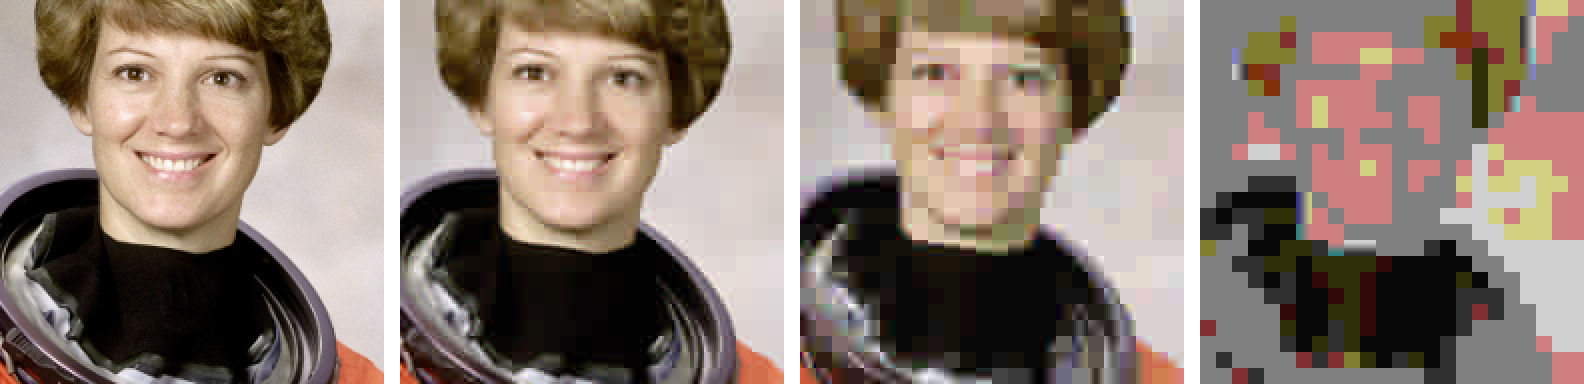
\includegraphics[width=0.585\textwidth]{figures/alpha.png}\hfill
  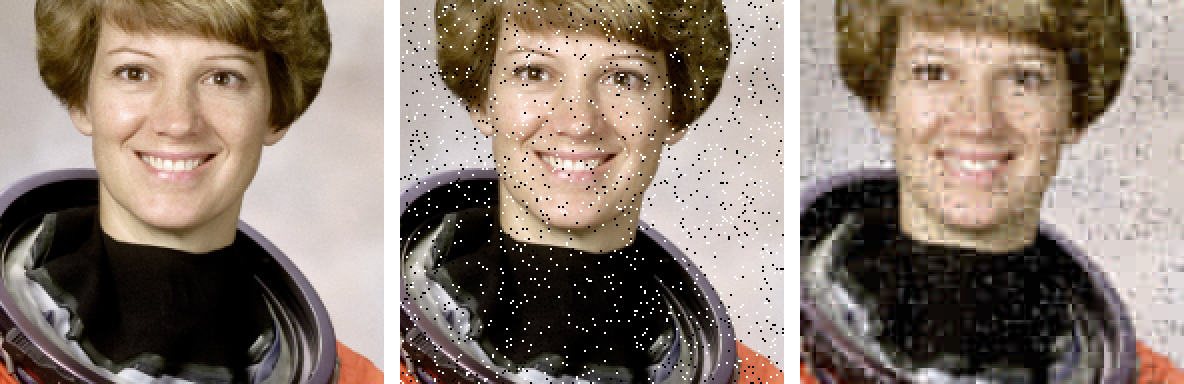
\includegraphics[width=0.395\textwidth]{figures/bruit.png}
  \caption{\small À gauche : originale, $\alpha = 1$, $5$ et $20$ (zoom). À droite : image
    pure, bruitée à 5\,\% (poivre et sel), reconstruite avec un masque triangulaire $F=4$.}
\end{figure}

Comme en MAM3, $\alpha$ règle le compromis entre taux et qualité : à $\alpha=20$,
presque tous les coefficients AC disparaissent et l'image devient une mosaïque de
blocs. La matrice uniforme garde 1,65\,\% des coefficients pour 13,9\,\% d'erreur,
quand la matrice psychovisuelle avec $\alpha=5$ en garde 2,15\,\% pour 11,3\,\% ; la
matrice qui privilégie les hautes fréquences conserve un quart des coefficients
pour une image moins fidèle. Avec 5\,\% de bruit poivre et sel, l'erreur par rapport à
l'image pure passe de 24,0\,\% (image bruitée) à 11,3\,\% après compression : la
troncature agit comme un filtre passe-bas, au prix d'un flou. \textbf{Performances :}
compression et décompression prennent 50\,ms en C++ contre 543\,ms en Python sur la
même machine (meilleur de trois essais), soit un facteur 11, grâce aux boucles
compilées en \code{-O2} au lieu d'appels numpy bloc par bloc.

\section{Bilan}
Le portage reproduit la version Python au coefficient près, aux arrondis flottants
près, et l'exécute onze fois plus vite. Les notions du cours ont guidé la structure :
les invariants rendent explicites des hypothèses implicites en Python (dimensions
multiples de 8, type \code{int16} des coefficients, cohérence d'un fichier CSR) et la
règle de zéro supprime toute gestion mémoire manuelle. Pistes : parcours zigzag et
codage entropique (RLE, Huffman) pour produire un vrai fichier JPEG, passage en
YCbCr, et stockage de plusieurs masques polymorphes avec \code{std::unique\_ptr}.

\end{document}
